\documentclass[11pt,oneside]{uhthesis}
\usepackage{subfigure}
% \usepackage[linesnumbered,lined,titlenumbered,ruled]{algorithm2e}
\usepackage[ruled,vlined,lined,linesnumbered,algochapter]{algorithm2e}
\usepackage{amsmath}
\usepackage{amssymb}
\usepackage{amsbsy}
\usepackage{mathpazo}
\usepackage{graphics}
\usepackage{float}
\usepackage{color}

%\usepackage{breqn}
\usepackage{listings}
\usepackage{xcolor}
 
\definecolor{codegreen}{rgb}{0,0.6,0}
\definecolor{codegray}{rgb}{0.5,0.5,0.5}
\definecolor{codepurple}{rgb}{0.58,0,0.82}
\definecolor{backcolour}{rgb}{0.95,0.95,0.92}
 
\lstdefinestyle{mystyle}{
    backgroundcolor=\color{backcolour},   
    commentstyle=\color{codegreen},
    keywordstyle=\color{magenta},
    stringstyle=\color{codepurple},
    basicstyle=\footnotesize,
    breakatwhitespace=false,         
    breaklines=true,                 
    captionpos=b,                    
    keepspaces=true,                 
    numbers=left,                    
    numbersep=5pt,                  
    showspaces=false,                
    showstringspaces=false,
    showtabs=false,                  
    tabsize=2
}
 
\lstset{style=mystyle}

%\floatstyle{ruled}
%\restylefloat{table}

\renewcommand{\tablename}{Tabla}
%\dontprintsemicolon

\title{Recuperación semántica de música utilizando embeddings y modelos de clasificación.}
\author{Niley González Ferrales}
\advisor{Dr. Yudivian Almeida}
\degree{Licenciado en Ciencia de la Computación}
\faculty{Facultad de Matemática y Computación}
\date{2024}
\logo{Graphics/uhlogo}
\makenomenclature

\renewcommand{\vec}[1]{\boldsymbol{#1}}
\newcommand{\diff}[1]{\ensuremath{\mathrm{d}#1}}

\begin{document}

\frontmatter
\maketitle

%\begin{flushright}
%{\it Es la historia de un hombre que cae de un edificio de cicuenta pisos. Para tranquilizarse mientras cae al vacío, no para de decirse: hasta ahora todo va bien, hasta ahora todo va bien, hasta ahora todo va bien. Pero lo importante no es la caída, es el aterrizaje.}

%\vspace{1cm}

%{\it C'est l'histoire d'un homme qui tombe d'un immeuble de 50 étages. Le mec, au fur et à mesure de sa chute, il se répète sans cesse pour se rassurer: <<Jusqu'ici tout va bien... Jusqu'ici tout va bien... Jusqu'ici tout va bien>>. Mais l'important, c'est pas la chute. C'est l'atterrissage.
	
%	{\bf La haine}}

%\vspace{1cm}

%A mi hermana, por acompañarme en la caída.

%A mis padres, por prepararme para el aterrizaje.
%\end{flushright}

\vspace*{5cm}
	\begin{flushright}
		A la ciencia.
		% {\it El que en lugar de chinchín, exija música; en lugar de placer, alegría; en lugar de dinero, alma; en vez de loca actividad, verdadero trabajo; en vez de jugueteo, pura pasión; para ese no es hogar este bonito mundo que padecemos...
			
		% 	\bfseries{El lobo estepario}}, {\bf Herman Hesse}
		
		% \vspace{1cm}
		
		% A mi hermana, por la alegría.
		
		% \vspace{0.5cm}
		
		% A mis padres, por el alma.
		
		% \vspace{0.5cm}
		
		% A Yadiel, por la pasión.
		
		% \vspace{0.5cm}
		
		% A mi tutor, por el verdadero trabajo.
		
		% \vspace{0.5cm}
		
		% A mis amigos, por la música.
	\end{flushright}
\begin{flushright}
	A la ciencia.\\
	\vspace{1cm}
	A los gigantes en cuyos hombros nos alzamos para elevar a la humanidad a nuevas alturas.
\end{flushright}
\chapter*{Opinión del tutor}


\vspace{1cm}

 \begin{flushright}
   \underline{\hspace{6.5cm}}\\
   Dr. Yudivian Almeida
   
   Facultad de Matemática y Computación
   
   Universidad de la Habana
   
   Enero, 2023
 \end{flushright}
\tableofcontents
\chapter*{Resumen}


{\bf Palabras claves:} 

\chapter*{Abstract}


{\bf Keywords:} 

\mainmatter
	
%===================================================================================
% Chapter: Introduction
%===================================================================================
\chapter{Introducción}
\label{chapter:introduction}
%===================================================================================
El auge de la tecnología digital, en los últimos años, ha llevado a una explosión en la cantidad de contenido multimedia accesible en línea. Incluyendo texto (libros, páginas web, ...), imágenes, videos y música; la red se ha convertido en un repositorio de información con un crecimiento vertiginoso \cite{owidinternet}. La necesidad de buscar en bases de datos cada vez más grandes ha impulsado importantes avances en el campo de la búsqueda y recuperación de información. Existen motores de búsqueda para diversos contenidos como páginas webs, imágenes y videos; sin embargo la música no es accesible de la misma forma \cite{Koepke2021AudioRW}. En este contexto, la presente tesis se propone explorar nuevas técnicas y enfoques para la búsqueda y recuperación de música en grandes bases de datos, con el objetivo de mejorar la accesibilidad de este recurso. \\

\section{Contexto histórico/social} 
\label{sec:context}

Durante las últimas décadas la tecnología computacional se ha desarrollado al punto de estar presente, de una manera u otra, en casi todos los procesos cotidianos de los seres humanos. La velocidad a la que se generan grandes volúmenes de datos (conocido comunmente como \textit{big data}), en la actualidad, desafía las capacidades de procesamiento computacional \cite{RiseofBigData}.\\
Una característica fundamental de estos volúmenes de datos es la gran variedad que presentan, siendo alrededor del 80$\%$ de naturaleza no estructurada. Y precisamente, la recuperación de información se define como encontrar resultados de naturaleza no estructurada que satisfaga una necesidad de información dentro de una gran colección de datos \cite{manning2008introductiontoIR}.\\
Los sistemas de recuperación de información (SRI) consisten en tecnologías y métodos diseñados para la búsqueda, almacenamiento, recuperación y organización de información. Estos sistemas son esenciales en la gestión de grandes cantidades de datos en diversos entornos, como bibliotecas digitales, bases de datos en línea y motores de búsqueda en la web.\\ 
La recuperación de información utilizando computadoras  se remonta a la década de 1950, y desde entonces se han desarrollado grandes ideas en el campo. Entre estas ideas se encuentran la creación de rankings de documentos, la representación vectorial de documentos y consultas, el agrupamiento de documentos similares, la asociación de términos con similitudes semánticas, la introducción de la frecuencia inversa en documentos y los modelos de semántica latente \cite{SRIConf1}.\\
Uno de los avances recientes en la recuperación de información es el uso de redes neuronales. Este es un campo que ha avanzado a pasos agigantados en la última década, en gran parte gracias al aumento del poder computacional introducido con las GPU. Los modelos de lenguaje, como Word2Vec \cite{Mikolov2013EfficientEO}, GloVe \cite{Pennington2014GloVeGV} y los más recientes, basados en \textit{transformers} \footnote{los \textit{transformers} son arquitecturas de aprendizaje profundo basadas en el mecanismo de autoatención. Se emplean, en especial, en el campo de procesamiento automático del lenguaje y visión artificial. Sus versiones más recientes se han utilizado predominantemente para entrenar grandes modelos de lenguaje en grandes datasets}, como BERT \cite{Devlin2019BERTPO} y GPT \cite{Radford2018ImprovingLU}, han demostrado una capacidad excepcional para capturar el significado semántico y la relación contextual entre palabras y frases. Estos modelos operan con representaciones de \textit{embeddings} a partir de diferentes enfoques cada uno.\\
Los embeddings son representaciones, en un espacio de relativamente baja dimensionalidad, de \textit{tokens} como frases, párrafos o documentos, a partir de un espacio vectorial de alta dimensionalidad, donde cada dimensión corresponde a una característica o atributo del lenguaje aprendido. Al aplicar estos \textit{embeddings} a la representación de documentos y consultas, se ha logrado una mejora significativa en la precisión y la relevancia de los resultados de recuperación de información \cite{docEmbReview}.\\ 

\section{Motivación}
\label{sec:motivation}

A pesar de que los SRI se han centrado principalmente en la recuperación de información con forma textual, se ha reconocido la necesidad de adaptar el entorno para manejar todo tipo de datos (como imágenes, videos, audios) \cite{JianMMIR}. La recuperación de información en datos no textuales presenta desafíos únicos, como la necesidad de comprender el contenido visual o auditivo de los datos. En el caso de imágenes, por ejemplo, la búsqueda puede basarse en características visuales como el color, la textura o la forma. En el caso de videos y audios, la búsqueda puede basarse en características como el tono, el ritmo o el contenido verbal. En los últimos años, ha habido avances significativos en la recuperación de información en datos no textuales, impulsados por el desarrollo de algoritmos de \textit{deep learning} y el aumento de la capacidad computacional. %; por ejemplo \cite{}$^n$.% TODO add referencia para justificar cuáles han sido esos avances significativos
Estos avances han permitido el desarrollo de sistemas más precisos y eficientes para la recuperación de imágenes, videos y audios.\\
Una herramienta utilizada comúnmente para recuperar información multimedia es representar los datos como texto, empleando metadatos \cite{Doh2022TowardUT}.
Estos metadatos sirven para describir y normalizar la representación de la información digital, lo que a su vez facilita su posterior búsqueda y recuperación. A pesar de sus beneficios, el uso de metadatos fijos conlleva limitaciones significativas como la imposibilidad de adaptarse a cambios en la información y la falta de precisión en la descripción de la información, así como la restricción a una cantidad limitada de información descriptiva. En este sentido, los metadatos fijos pueden resultar insuficientes para abarcar la complejidad inherente a la información multimedia, lo que a su vez puede dificultar su precisa recuperación. \\
La creación de metadatos suele requerir un enfoque manual o, en su defecto, la utilización de modelos de inteligencia artificial. Sin embargo, estos modelos, al depender de los datos con los que fueron entrenados, sufren dificultades para generalizar adecuadamente para contextos específicos. Además, la naturaleza dinámica de la información multimedia puede llevar a que los metadatos fijos se vuelvan obsoletos con el tiempo, lo que impacta negativamente la precisión y exhaustividad en la recuperación de información. \\ % TODO cite somewhere in this text
Dadas las limitaciones que presenta la recuperación utilizando metadatos, se han estudiado otras alternativas. Un ejemplo es la consulta por tarareo (\textit{query-by-humming}) o la consulta por ejemplo (\textit{query-by-example}), en la que la consulta se representa mediante una grabación de audio y el sistema recupera la canción correcta (la más similar). La recuperación basada en contenido consiste en buscar audio que coincida con una consulta de audio. Dado un audio de ejemplo, se devuelven los audios más similares en la base de datos. Sin embargo, satisfacer los requisitos para introducir un audio puede resultar difícil para los usuarios. Por otro lado, las consultas detalladas en lenguaje natural con forma libre constituyen una interfaz familiar ampliamente utilizada en los motores de búsqueda actuales, lo que permite solicitar música con información semántica.\\
Permitir a los usuarios buscar música utilizando oraciones en lenguaje natural introduce una capa adicional de complejidad, ya que requiere el puente entre la semántica del lenguaje y la representación de la música en sí misma.\\
%% Actualidad, novedad científica e importancia teórica y práctica
Uno de los desafíos clave en la integración del lenguaje natural y análisis de audios en los SRI se encuentra en la representación efectiva de la música en función de las consultas textuales. Hasta donde se ha podido comprobar, este problema no ha sido abordado utilizando las emergentes capacidades semánticas y contextuales de los grandes modelos de lenguajes (LLM por sus siglas en inglés). Tampoco se ha observado una estrategia de caracterización de la música empleando modelos pre-entrenados de inteligencia artificial, como una alternativa a entrenar modelos de \textit{music captioning} que son la forma más directa de representar música como texto. Depender de un único modelo trae desventajas en cuanto a que las características que se pueden extraer, están limitadas a las que aparecen en los datos de entrenamiento; esas desventajas son acentuadas por el conocido problema que hay con la indisponibilidad de \textit{datasets} de tamaño adecuado y con amplio rango de modalidades \cite{Simonetta2019MultimodalMI}. \\

\section{Antecedentes}
\label{sec:anteced}

Este trabajo es pionero en la investigación de recuperación semántica de música en la Facultad. No se cuentan con investigaciones en esta área. 

\section{Problemática}
\label{sec:problem}

Durante una exahustiva investigación no se encontró ningún sistema o diseño que permita organizar y recuperar música de una gran base de datos utilizando consultas en lenguaje natural y con componentes semánticos y que, además, sea escalable respecto a las características(o \textit{features}) que se conocen de la música. \\
%% - objetivo general
\section{Objetivos}
\label{sec:objective}

El objetivo de esta investigación es el diseño e implementación de un prototipo de una plataforma que permita realizar consultas en lenguaje natural sobre una base de datos de música y obtener resultados con significación semántica.\\
%% - objetivos específicos para cumplir el objetivo general
Los objetivos específicos planteados para dar cumplimiento al objetivo general son:
\begin{itemize}
    \item Estudiar los resultados más recientes relacionados con recuperación de información multimedia, en particular de música. Indagando en recuperación con consultas en lenguaje natural.
    \item Modelar un sistema de extracción de \textit{features} que sea flexible, permitiendo actualizar y añadir información sobre la música.
    \item Modelar un SRI que devuelva canciones relevantes a consultas en lenguaje natural. Intentando incluir similitud semántica sin sacrificar mucha eficiencia.
    \item Implementar la plataforma modelada anteriormente.
    \item Evaluar el Sistema de Recuperación y comparar los resultados con modelaciones similares en la literatura.
    \item Realizar una página web utilizando django \textit{framework} que permita escribir consultas y reproducir la música que sea resultado de la consulta; como interfaz para probar el prototipo implementado.
    % \item Crear un \textit{framework} que permita extraer características de una canción y que sea extensible respecto a los modelos de extracción de características.
    % \item Crear un software que utilizando grandes modelos de lenguaje convierta los características extraídas, en un texto coherente y sin alucinaciones. 
    % \item Crear un SRI con un modelo similar al modelo vectorial, pero utilizando como vectores los \textit{embeddings} de las consultas y textos (empleando BERT).
\end{itemize}
% \section{Propuesta de solución} % optional, kinda
% Para cumplir con los objetivos planteados se propone

%% - pregunta ciéntifica
%\section{Preguntas ciéntificas}
%\label{sec:questions}
%A través del documento se abordarán las siguientes preguntas con la intención de resolver el problema planteado:
%\begin{itemize}
%    \item ¿Un \textit{framework} escalable conformado por modelos de \textit{Music Information Retrieval}(MIR) de clasificación de música es, al menos, igual de efectivo al extraer características de música, que los modelos existentes de \textit{auto-tagging} o \textit{captioning}?
%    \item ¿Se puede diseñar un sistema de recuperación que utilice las características extraídas (que son básicamente metadatos), pero sin las limitaciones que conllevan?  % ¿Es posible convertir una estructura de datos con las características de una canción en un texto descriptivo, similar al resultante de hacer \textit{captioning}, pero utilizando LLMC?
%    % \item ¿Qué problemas puede traer la propensión a alucinar de dichos LLM para esta tarea?
%    \item ¿Un SRI utilizando \textit{embeddings} es más efectivo en cuánto a similitud semántica que empleando vectores de bolsa de palabras? % semántica latente no es factible por el enorme costo computacional que tiene, que empeora con el tamaño del corpus, y bueno, queremos analizar grandes bases de datos. 
%\end{itemize}

%% - estructura del trabajo
\section{Estructura de la tesis}
\label{sec:structure}

A continuación se describe la estructura del documento.  En el capítulo \ref{chap:sota}, \textbf{Estado del Arte}, se define el marco teórico del trabajo, que abarcará los modelos de recuperación de información, los acercamientos a recuperación de audios y música, modelos de lenguaje y como sobreponerse al \textit{semantic gap}. En el capítulo \ref{chap:design-implem}, \textbf{Diseño e implementación}, se presenta la modelación de la propuesta para atacar el problema planteado y se describen los detalles de implementación incluyendo las alternativas que no se pudieron comprobar. Finalmente, en el capítulo \ref{chap:experiment}, \textbf{Breve Experimentación}, se muestran las evaluaciones del modelo de recuperación. A continuación aparecen las \hyperref[chap:conclusions]{\textbf{Conclusiones}} y las \hyperref[chap:recommendations]{\textbf{Recomendaciones}}. El documento finaliza con la \textbf{Bibliografía}.

%===================================================================================
% Chapter: State of the Art
%===================================================================================
\chapter{Estado del Arte}
\label{chap:sota}
%===================================================================================

Este trabajo se relaciona con varios temas en la literatura: procesamiento y recuperación de información musical, recuperación de música basada en texto, brecha semántica, procesamiento de lenguaje natural en Recuperación de Información Musical (MIR, por sus siglas en inglés), descripción de música (\textit{music captioning}), aprendizaje a partir de supervisión de lenguaje y \textit{embeddings} en recuperación de información.\\

\section{Procesamiento y recuperación de información musical}
\label{sec:MIR}

El campo de investigación de MIR se ocupa de la extracción e inferencia de características significativas de la música (ya sea desde las señales de audio, representación simbólica o fuentes externas como páginas web), indexando la música usando estas características y desarrollando diferentes esquemas de búsqueda y recuperación (por ejemplo, búsqueda basada en contenido, sistemas de recomendación musical o interfaces de usuario para explorar grandes colecciones de música) \cite{Schedl2014MusicIR}.

La música es un artefacto humano altamente multimodal. En este caso, por modalidad, se refiere a una forma específica de digitalizar la información musical \cite{Simonetta2019MultimodalMI}. Diferentes modalidades se obtienen a través de diferentes transductores, en diferentes lugares o momentos, y/o pertenecen a diferentes medios. Ejemplos de modalidades que pueden asociarse a una sola pieza de música incluyen audio, letras, partituras simbólicas, portadas de álbumes, y así sucesivamente \cite{Simonetta2019MultimodalMI, Schedl2014MusicIR}.

Los enfoques computacionales en MIR típicamente emplean características y crean modelos para describir la música por una o más de las siguientes categorías de percepción musical: contenido musical, contexto musical, propiedades del usuario y contexto del usuario, como se define en \textit{Music Information Retrieval: Recent Developments and Applications} \cite{Schedl2014MusicIR}. Se hace referencia al contenido musical como los aspectos codificados en la señal de audio, tales como: ritmo, melodía, volumen, letras de canciones y timbre. Mientras que el contexto musical se define como factores que no pueden extraerse directamente del audio, pero que están relacionados, no obstante, con el ítem musical, el artista o el intérprete. Al centrarse en el usuario, los aspectos del contexto del usuario representan factores dinámicos y frecuentemente cambiantes, y las propiedades del usuario se refieren a características constantes o de cambio lento, como sus gustos musicales o educación musical.

Es importante señalar que existen interconexiones entre algunas características de diferentes categorías. Por ejemplo, los aspectos reflejados en el contexto musical (por ejemplo, el género musical) pueden ser modelados por el contenido musical (por ejemplo, la instrumentación).

\textbf{Aplicaciones de procesamiento y recuperación de información musical}
\begin{itemize}
    \item La recuperación de música tiene la intención de ayudar a los usuarios a encontrar música en grandes colecciones según un criterio particular de similitud. En \textit{query-by humming} (búsqueda por tarareo) y \textit{query-by example} (búsqueda mediante ejemplo), el objetivo es recuperar música a partir de una entrada melódica o rítmica dada. Se basan en la comparación de una señal musical objetivo con una base de datos, pero los usuarios pueden querer encontrar música que cumpla con ciertos requisitos (por ejemplo, "dame canciones con un tempo de 100 bpm o en do mayor") \cite{Schedl2014MusicIR}. De hecho, las personas generalmente usan etiquetas o descripciones semánticos (como `alegre'  o `rock') para referirse a la música. 
    \item El alineamiento o sincronización de audio es un escenario similar a la recuperación de música donde, además de identificar un fragmento de audio dado, el objetivo es conectar localmente, posiciones temporales de dos señales musicales.
    \item Los sistemas de recomendación de música suelen proponer una lista de piezas musicales basándose en modelar las preferencias musicales del usuario.
    \item La generación automática de listas de reproducción está relacionada con la recomendación de música. Su objetivo es crear una lista ordenada de resultados, como pistas musicales o artistas, para proporcionar listas de reproducción significativas y agradables para el oyente. Una de las diferencias entre la recomendación de música y la generación de listas de reproducción es que la primera suele proponer nuevas canciones no conocidas por el usuario, mientras que la segunda tiene como objetivo reorganizar material ya conocido.
\end{itemize}

\textbf{Tareas de procesamiento y recuperación de información musical}
\begin{itemize}
    \item Extracción de características del contenido y contexto musical. Las características de audio pueden subdividirse en físicas y perceptuales \cite{Alas2016ARO}. Las físicas, que pueden calcularse en diversos dominios como el tiempo, la frecuencia o la wavelet, incluyen \textit{zero-crossing rate}, la amplitud, el ritmo, basadas en autoregresión, basadas en STFT (Transformada de Fourier de Tiempo Corto), brillo, tonalidad, croma y forma del espectro. Por otro lado, las características perceptuales intentan integrar el procesamiento de percepción del sonido humano. Por ejemplo, los Coeficientes Cepstrales de Frecuencia Mel (MFCC), paquetes de wavelets perceptuales, y la intensidad sonora.
    \item La similitud es la tarea de calcular la la semejanza entre el contenido de la información. A menudo, esta tarea tiene el propósito de recuperar documentos de una colección a través de una consulta, que puede ser explícitamente expresada por el usuario o deducida implícitamente por el sistema \cite{Simonetta2019MultimodalMI}. Un ejemplo muy común de consultas de similitud explícita es la búsqueda por ejemplo, en la cual la consulta está representada por una grabación de audio y el sistema recupera la canción correcta. Por otro lado, las consultas implícitas se utilizan en sistemas de recomendación y generadores de listas de reproducción.
    \item La clasificación consiste en tomar como entrada una pieza musical y devolver una o más etiquetas. Una tarea de clasificación popular es el reconocimiento del estado de ánimo o la emoción \cite{Kim2010StateOT}, mientras que una emergente es la clasificación de género \cite{Allamy20211DCA, AthulyaK2021DeepLB, Qiu2021DBTMPEDB, Rafi2021ComparativeAO, Koparde2021ASO, Ndou2021MusicGC, Prince2022MusicGC}. Ambas tareas pueden aprovechar grabaciones de audio, letras, portadas y metadatos. Otras tareas de clasificación incluyen: clasificación de instrumentos, clasificación de obras derivadas, identificación de tonos y descripción musical expresiva.
\end{itemize}

\section{Recuperación de música basada en texto}
\label{sec:text-based retrieval}

Con el paso de los años se han propuesto numerosos enfoques para navegar, buscar y descubrir música a través de una variedad de interfaces \cite{Manco2022ContrastiveAL}. Más allá de la búsqueda simple por metadatos, los sistemas de recuperación de música permiten expresar consultas a través de letras \cite{Tsukuda2017LyricJA}, ejemplos de audio \cite{Lee2020DisentangledMM}, videos \cite{Li2019QueryBV} y tarareos \cite{Patel2021MusicRS}, entre otros.

A pesar de que cada uno de estos tipos de consulta tiene sus méritos, ninguno de ellos admite una de las formas más populares de buscar en la actualidad: mediante texto libre. Por ejemplo, comúnmente buscamos canciones escribiendo texto en un motor de búsqueda o preguntando a comunidades en línea para identificar una pieza de música de la que no tenemos información bibliográfica o editorial. Habilitar a los sistemas MIR para interpretar consultas en lenguaje natural puede tener beneficios de gran alcance \cite{Manco2022ContrastiveAL}.

Un sistema de recuperación basado en texto ideal necesita ser flexible para permitir varios tipos de entrada (como palabras, oraciones) y tener vocabularios abundantes. Por ejemplo, se pueden utilizar etiquetas populares como el género, para explorar la biblioteca musical. A veces, las consultas de entrada pueden incluir tipos de etiquetas musicales no vistas anteriormente. Además, uno puede utilizar descripciones más detalladas a nivel de oración para descubrir música. % TODO rephrase

La recuperación basada en texto es desafiante porque necesita manejar, no solo metadatos editoriales (título, artista, año de lanzamiento), sino también información semántica (género, estado de ánimo, tema). Además, los sistemas modernos de recuperación, como los asistentes de voz, necesitan generalizar a entradas de lenguaje natural a nivel de oración; más allá de vocabularios con etiquetas fijas \cite{Doh2022TowardUT}.

Otro enfoque reciente para la recuperación de información (IR) es a través de modelos neuronales de ranking, que utilizan redes neuronales superficiales o profundas. Los modelos tradicionales de aprendizaje de clasificación emplean técnicas de aprendizaje automático sobre \textit{features} hechos a mano. En contraste, los modelos neuronales aprenden representaciones del lenguaje a partir de texto puro; que pueden disminuir la brecha entre el vocabulario de la consulta y el del documento \cite{Mitra2017NeuralMF}.

Desde el comienzo de la década, ha habido mejoras dramáticas en el rendimiento en tareas de visión por computadora, reconocimiento de voz y traducción automática, tanto en la investigación como en aplicaciones del mundo real \cite{LeCun2015DeepL}. Estos avances han sido propulsados en gran medida por los recientes progresos en modelos de redes neuronales, generalmente con múltiples capas ocultas, conocidos como arquitecturas profundas (\textit{deep learning}) \cite{LeCun2015DeepL, Bahdanau2014NeuralMT, Deng2014DeepLM, Hinton2012DeepNN}. 

Los modelos neuronales para IR utilizan representaciones vectoriales de texto y suelen contener una gran cantidad de parámetros que necesitan ser ajustados. Los modelos de aprendizaje automático (machine learning, ML) con un gran conjunto de parámetros suelen requerir una gran cantidad de datos de entrenamiento \cite{Taylor2006OptimisationMF}.

El aprendizaje de representaciones adecuadas de texto, también requiere datasets a gran escala durante el entrenamiento \cite{Mitra2016LearningTM}. Por lo tanto, a diferencia de los modelos clásicos de IR, estos enfoques neuronales tienden a requerir muchos datos; mejorando su rendimiento con la cantidad de datos de entrenamiento \cite{Mitra2017NeuralMF}.

Los enfoques más similares a esta investigación son los estudios en MusCALL \cite{Manco2022ContrastiveAL} y MuLan \cite{Huang2022MuLanAJ}, que utilizan aprendizaje contrastivo cruzado y multimodal para crear un espacio compartido de \textit{embeddings} o \textit{embeddings} multimodales. Publicado en noviembre de 2022, \textit{Toward Universal Text-To-Music Retrieval} \cite{Doh2022TowardUT} ahonda en un estudio de diseños efectivos para sistemas de recuperación de texto-música, proponiendo un sistema universal de recuperación de texto-música, que logra un rendimiento de recuperación comparable tanto en consultas a nivel de \textit{tags} como a nivel de oraciones.

\section{Brecha semántica}
\label{sec:semantic-gap}

La brecha semántica (\textit{semantic gap}) en la recuperación de música se refiere a la diferencia entre descripciones acústicas de bajo nivel y conceptos humanos de alto nivel (significativos para la percepción musical humana). Por ejemplo, el mismo tempo puede aparecer en diferentes géneros musicales, y un género musical dado puede estar caracterizado por diferentes tempos \cite{Su2022HighperformanceCM}.

Esta brecha existe porque las características que los ordenadores pueden analizar, como el tono, el tempo y el volumen, no son los mismos que los conceptos que los humanos utilizan para relacionarse con colecciones de música \cite{Celma2006BridgingTM}. Idealmente, los enfoques de recuperación y recomendación de música deberían incorporar aspectos de varias categorías para superar la brecha semántica \cite{Schedl2014MusicIR}.

Un enfoque multimodal para superar la brecha semántica en la música implica combinar diversas técnicas y fuentes de datos para mejorar la precisión de los sistemas de recuperación y recomendación de música \cite{Celma2006AMA}.

\section{Procesamiento de Lenguaje Natural en MIR}
\label{sec:NLP_in_MIR}

El Procesamiento de Lenguaje Natural (NLP, por sus siglas en inglés) es un campo de la Ciencia de la Computación y la Inteligencia Artificial, que se ocupa de la interacción entre las computadoras y el lenguaje humano (natural) \cite{NLP4MIR}. El NLP es un componente fundamental en tecnologías de la vida diaria: búsqueda en la web, reconocimiento y síntesis de voz, resúmenes automáticos en la web, recomendación de productos (incluida la música), traducción automática, entre otros.

Trabajos previos en la literatura de MIR han explorado aprovechar NLP en el ámbito musical desde diferentes enfoques. Los esfuerzos iniciales se centraron en el texto como una modalidad aislada, adoptando técnicas para construir bases de conocimiento a partir de corpus de texto relacionados con la música \cite{Oramas2016InformationEF}, o construir grafos semánticos para la similitud entre artistas a partir de biografías \cite{Oramas2015ASA}. Los esfuerzos recientes han comenzado a favorecer, en cambio, enfoques multimodales. Estos han explorado el aprendizaje profundo con datos de entrada multimodales, típicamente audio combinado con texto, como reseñas o letras, para aplicaciones tan variadas como la clasificación y recomendación musical \cite{Oramas2018MultimodalDL}, detección de estado de ánimo \cite{Delbouys2018MusicMD}, reconocimiento de emociones en la música \cite{Jeon2017MusicER} y descripción de música (captioning) \cite{Manco2021MusCapsGC, Cai2020MusicAA}.

Por otro lado, la idea de permitir que los sistemas de MIR interpreten consultas en lenguaje natural no es nueva; algunos trabajos, como el de Brian Whitman y Ryan M. Rifkin \cite{Whitman2002MusicalQA}, han sugerido direcciones de investigación similares. Sin embargo, hasta recientemente, los sistemas multimodales que integran lenguaje natural no han sido ampliamente adoptados dentro de la comunidad de MIR, posiblemente debido a la falta de datasets adecuados o a las limitaciones prácticas de los métodos de NLP anteriores a los modelos de lenguaje modernos \cite{Manco2022ContrastiveAL}. A la luz de los avances recientes en modelos de lenguaje, se argumenta que el aprendizaje audio-lenguaje tiene el potencial de cerrar la brecha semántica en MIR.

\section{Descripción de música}
\label{sec:music_captioning}

\textit{Music captioning} se define como la tarea de generar una descripción en lenguaje natural del contenido de audio de la música de una manera humana.
MusCaps \cite{Manco2021MusCapsGC} en 2021, afirman presentar el primer modelo de \textit{music audio captioning}. Hasta hace poco, los enfoques en MIR para la descripción de música normalmente se basaban en clasificación de una o múltiples etiquetas. Un ejemplo destacado es el \textit{auto-tagging} de música \cite{Choi2016AutomaticTU, Lee2017SamplelevelDC, Pons2017EndtoendLF}, en el cual se asignan \textit{tags} descriptivos a un fragmento musical para transmitir características de alto nivel de la entrada, como género, instrumentación y emoción.

Los sistemas de \textit{captioning} necesitan reconocer características a nivel de señal como la instrumentación y descriptores de alto nivel como el género. También producen oraciones descriptivas completamente formadas que se asemejan más a las consultas humanas. A través del uso conjunto y procesamiento de información auditiva y lingüística, \textit{music captioning} representa un primer paso hacia el desarrollo de modelos de audio y lenguaje para la comprensión musical. Finalmente, la descripción de música tiene varias aplicaciones directas, como habilitar la búsqueda de música a través de consultas más naturalmente humanas, o proporcionar explicaciones para recomendaciones automáticas de música \cite{Manco2021MusCapsGC}.

El estudio \textit{Audio Retrieval with Natural Language Queries: A Benchmark Study} \cite{Koepke2021AudioRW} se centra en la recuperación de eventos de audio (no musicales) mediante consultas en lenguaje natural. Considerando que aprender (en el sentido de  \textit{machine learning} ) a recuperar audio con consultas en lenguaje natural requiere datos con texto y sonido emparejados, ellos \cite{Koepke2021AudioRW} afirman que los datasets de \textit{audio captioning} se prestan naturalmente a esta tarea, ya que contienen audio y una descripción de texto correspondiente al sonido. Proponen aprender \textit{cross-modal embeddings} utilizando datasets de \textit{audio captioning} para el sistema de recuperación. Varios estudios en recuperación de música con consultas en lenguaje natural mencionan esta idea con datasets de \textit{music captioning} \cite{Doh2022TowardUT, Manco2022ContrastiveAL, Huang2022MuLanAJ}. Sin embargo, también se señala que los datasets existentes actualmente no abarcan la diversidad del lenguaje descriptivo del sonido \cite{Huang2022MuLanAJ}; mientras que algunos estudios terminan utilizando una concatenación de \textit{tags} de diferentes fuentes de anotación como \textit{captions} \cite{Doh2022TowardUT}.

\section{Aprendizaje a partir de Supervisión de Lenguaje}
\label{sec:learning_lang_superv}

El aprendizaje multimodal todavía ocupa un papel marginal en MIR y aún no ha disfrutado completamente de los beneficios de los modelos de lenguaje modernos \cite{Manco2022ContrastiveAL}. La idea clave detrás de estos modelos es que el lenguaje captura muchas de las abstracciones que los humanos utilizan para navegar por el mundo y, por lo tanto, puede actuar como supervisión para el aprendizaje de propósito general, incluso en tareas que no se basan directamente en el lenguaje.

Los clasificadores generalmente se entrenan para etiquetar ejemplos, con clases predefinidas y fijas. Impulsados por los avances recientes en modelación neuronal de lenguaje y su competencia demostrada en aprendizaje por transferencia, los investigadores han comenzado a explorar menos restrictivas interfaces de lenguaje natural, para acceder a la información categórica subyacente a las señales sin procesar \cite{Huang2022MuLanAJ}. La mayoría de ese trabajo se ha centrado en el dominio de eventos visuales y de audio, combinando contenido multimedia con subtítulos en lenguaje natural \cite{Koepke2021AudioRW, Jia2021ScalingUV, Radford2021LearningTV, Nagrani2022LearningAM}.

El éxito de estos esfuerzos depende en gran medida de recursos de entrenamiento a gran escala y de arquitecturas de redes neuronales robustas, que sean lo suficientemente flexibles para modelar la compleja y no monótona relación entre el lenguaje y otras modalidades. En particular, el dominio visual ha obtenido grandes beneficios de la disponibilidad de grandes cantidades de imágenes con descripciones disponibles en la web \cite{Jia2021ScalingUV}. Sin embargo, en el dominio general de audio ambiental, pares de audio-descripción a gran escala están menos disponibles y los esfuerzos relacionados se han basado pequeños datasets de \textit{captions} \cite{Drossos2019ClothoAA, Kim2019AudioCapsGC}.

\section{\textit{Embeddings} en recuperación de información}
\label{sec:semantic_embedd}

Un \textit{embedding} es una representación de elementos en un nuevo espacio, de manera que se preservan las propiedades y relaciones entre los elementos. El objetivo de un \textit{embedding} es generar una representación más simple, donde la simplificación puede implicar una reducción en el número de dimensiones, un aumento en la dispersión de la representación, desentrañar los componentes principales del espacio vectorial, o una combinación de estos objetivos \cite{Mitra2017NeuralMF}.

Los \textit{embeddings} de palabras, de modelos pre-entrenados, se utilizan en diversas aplicaciones, como en la construcción de representaciones para frases, párrafos y documentos \cite{Brundha2022VectorMB}. Con modelos de \textit{embedding} de palabras, los documentos preprocesados se mapean a vectores de números reales mediante tecnologías como redes neuronales, reducción de dimensionalidad en la matriz de co-ocurrencia de palabras, entre otras \cite{Yuan2020ImprovingIR}.\\
Dado que tienen en cuenta el contexto donde aparecen las palabras, permite la predicción de palabras faltantes en un documento. En contraste, los motores de búsqueda tradicionales, basados en palabras clave, no pueden resolver el problema de la alta discrepancia entre términos; y considerar las diferencias de significado entre palabras semánticamente similares en el proceso de comparación. 

Los modelos de \textit{embeddings} más utilizados/estudiados en la literatura incluyen:
\begin{itemize}
    \item \textbf{Word2vec} \cite{Mikolov2013EfficientEO} (2013): es un conjunto de modelos relacionados que se utilizan para producir \textit{embeddings} de palabras. Estos modelos son redes neuronales superficiales de dos capas que se entrenan para reconstruir contextos lingüísticos de palabras. Word2vec puede utilizar dos arquitecturas de modelo para producir estas representaciones distribuidas de palabras: \textit{Continuous Bag-Of-Words} (CBOW) o \textit{skip-gram} de deslizamiento continuo. En ambas arquitecturas, word2vec considera tanto palabras individuales como una ventana de contexto deslizante a medida que itera sobre el corpus. El problema de la dispersión en word2vec causa que la dimensión de su espacio vectorial sea mayor que otras tecnologías, lo que provoca un uso excesivo de recursos de memoria y una baja robustez \cite{Yuan2020ImprovingIR}.
    \item \textbf{GloVe} \cite{Pennington2014GloVeGV} (2014): acuñado a partir de su nombre en inglés \textit{Global Vectors}, es un algoritmo de aprendizaje no supervisado para obtener representaciones vectoriales de palabras. Resulta en un modelo global de regresión log-bilineal que combina las ventajas de las dos principales familias de modelos en la literatura: factorización de matrices globales y métodos locales de ventana de contexto.
    \item \textbf{BERT} \cite{Devlin2019BERTPO} (2019): abreviatura de \textit{Bidirectional Encoder Representations from Transformers}, es un modelo de lenguaje basado en la arquitectura \textit{transformer}, notable por su mejora dramática respecto a anteriores modelos en el estado del arte. El modelo pre-entrenado de BERT puede ser ajustado (\textit{fine-tuning}) con solo una capa de salida adicional, para crear modelos de última generación para una amplia gama de tareas; como respuesta a preguntas e inferencia de lenguaje, sin modificaciones sustanciales en la arquitectura específica de la tarea. \textit{Sentence BERT} (SBERT) \cite{Reimers2019SentenceBERTSE} es un algoritmo basado en aprendizaje automático que utiliza un \textit{transformer} de oraciones para generar \textit{embeddings} de oraciones mediante una red neuronal siamesa. SBERT puede ser beneficioso para la búsqueda semántica y la similitud textual semántica.
\end{itemize}

Los sistemas de recuperación de información basados en \textit{embeddings} reciben una entrada del usuario en forma de consulta. Luego, el sistema procesa todas las consultas y genera \textit{embeddings} vectoriales que ayudan a comparar la consulta con la colección de documentos del corpus. Los \textit{embeddings} de la consulta y del documento pueden compararse utilizando una variedad de métricas de similitud, como la similitud del coseno o el producto punto. Los documentos relevantes se envían al usuario en orden decreciente de relevancia, lo que ayuda a identificar cuáles resultados son mejores.

\section{Datasets}
\label{sec:datasets}

Para establecer un baseline de la eficacia del prototipo a implementar es necesario evaluarlo con las métricas usuales en SRI y preferentemente en el mismo conjunto de datos que otros trabajos en el tema. 

\textit{Contrastive Audio-Language Learning for Music} \cite{Manco2022ContrastiveAL} entrenaron y evaluaron su modelo de recuperación en un dataset de 250 mil pares (audio, texto) creado a partir de una biblioteca de música en producción. Pero no se encuentra disponible públicamente para utilizarlo y comparar justamente los resultados.

La evaluación de recuperación de música a partir de consultas textuales de \textit{MuLan: A Joint Embedding of Music Audio and Natural Language} \cite{Huang2022MuLanAJ} fue una colección patentada de 7,000 listas de reproducción curadas por expertos. Que tampoco fue encontrada públicamente.

Dado la idea mencionada en la sección \ref{sec:music_captioning}, se decidió encontrar un dataset de \textit{music captioning}. Sin embargo la mayoría de los utilizados en la literatura son privados. Finalmente se optó por utilizar MusicCaps \cite{Agostinelli2023MusicLMGM}, que fue liberado públicamente por \textit{Google} en una investigación de hace apenas unos meses. 

En \textit{HuggingFace} \cite{huggFaceMusicCaps} aparece una descripción del dataset, el .csv y  un \textit{script} \footnote{\href{https://github.com/nateraw/download-musiccaps-dataset}{https://github.com/nateraw/download-musiccaps-dataset}}  para descargar los clips de YouTube. MusicCaps contiene 5,521 clips de 10 segundos, extraídos de AudioSet \cite{Gemmeke2017AudioSA}. Por cuestiones de conectividad, para esta investigación se utiliza un subconjunto de clips, lo que no causa ningún problema dado que no es necesario tener una cantidad de datos específica con que entrenar. Cada clip contiene una lista de 'aspectos' (\textit{aspect list}) y una descripción textual escrita por músicos. \\
Una lista de aspectos es, por ejemplo, "\textit{pop, tinny wide hi hats, mellow piano melody, high pitched female vocal melody, sustained pulsating synth lead}". \\
Mientras que la descripción consta de varias oraciones sobre la música como, " \textit{A low sounding male voice is rapping over a fast paced drums playing a reggaeton beat along with a bass. Something like a guitar is playing the melody along. This recording is of poor audio-quality. In the background a laughter can be noticed. This song may be playing in a bar.} "

La escasez de datasets en MIR es un gran obstáculo en el desarrollo del campo. Se debe, en parte, a que a diferencia de otros tipos de multimedia, la música tiende a tener \textit{copyright} más estricto. Lo que impide crear conjuntos de datos con ejemplos representativos, que además sean lo suficientemente grandes para ser útiles en las arquitecturas de redes neuronales utilizadas en el presente para aprender en el campo de texto o imágenes, por ejemlo. Esto ha implicado que varias investigaciones recientes, incluyendo la presente, decidan apoyarse en las capacidades de transferencia de conocimiento que poseen los modelos de lenguaje, como fue explicado en la sección \ref{sec:learning_lang_superv}, para tareas en MIR que incluyan trabajo con texto.

%===================================================================================
% Chapter: Design and implementation
%===================================================================================
\chapter{Diseño e implementación}
\label{chap:design-implem}
%===================================================================================
\section{Modelo general}
\label{sec:design}
El primer paso consiste en definir qué método utilizar para obtener una representación de la música (sobreponiéndose a la brecha semántica), que pueda ser utilizada para la recuperación semántica con consultas textuales.

Una de las estrategias de recuperación de información (con consultas textuales) utilizada extensamente, como se ha mencionado anteriormente, es mediante metadatos. Se debe recordar que dicha estrategia requiere que las canciones contengan metadatos curados (que no es muy práctico en los escenarios actuales donde la multimedia se genera en grandes cantidades, y libremente). Además, como segunda desventaja, la información conocida sobre las canciones estaría limitada al conjunto fijo de metadatos que se predefinan. 

Si se extraen los metadatos (\textit{tags}, \textit{features}) automáticamente con modelos de \textit{Machine Learning} de clasificación y auto-tagging, se hace frente al primer problema mencionado: cómo hacer que todas las canciones tengan metadatos, sin requerir una cantidad de trabajo humano irrealista. Dado que los \textit{tags} se extraen automáticamente, se abre una ventana a contrarrestar la segunda desventaja, ya que la cantidad de tags dependería de la cantidad de modelos de \textit{Machine Learning}. Esto incluso permite que el conjunto no sea fijo. Con el costo de reprocesar la base de datos, se hace posible actualizar y añadir valores.

Otra estrategia, que ha sido analizada por las escasas investigaciones en el tema, es diseñar un modelo para convertir la música al espacio del lenguage natural, o convertir las descripciones textuales y la música a un espacio compartido. El problema fundamental de este acercamiento es que requiere un conjunto bastante grande de pares texto-música, lo suficientemente diverso y abarcador para maximimar la generalización del modelo. La inexistencia de dichos datasets \cite{Simonetta2019MultimodalMI, Huang2022MuLanAJ, Manco2022ContrastiveAL}, en conjunto con las dificultades de requerimientos computacionales; no permiten realizar el entrenamiento necesario para implementar esta estrategia. 

La propuesta de extraer los \textit{features} automáticamente trabaja bajo la premisa de que el campo de MIR se ha desarrollado en tareas de clasificación y auto-tagging lo suficiente para ser competitivo con metadatos hechos a mano, relativo al esfuerzo que conlleva cada uno. % TODO specify a little more on our proposal

Para garantizar que el sistema de recuperación tenga en cuenta la similitud semántica, se propone utilizar un acercamiento con \textit{Sentence BERT} (sec. \ref{sec:semantic_embedd}) para comparar las consultas con las descripciones de la música. Los enfoques tradicionales en SRI para mantener la significación semántica, suelen requerir estructuras complejas y un largo tiempo de preprocesamiento o de ranking (como Latent Semantic Analysis (LSA) \cite{Foltz1996LatentSA}). Con el auge de los modelos de lenguaje (alrededor de los últimos de cinco años) y su capacidad de capturar significado semántico y relación contextual; se ha abierto el camino para combinar la eficiencia del modelo vectorial con bolsa de palabras y el aumento en precisión de los modelos como LSA. 
% TODO explain the relationship between language models and the combination 

Dado que SBERT captura el \textit{embedding} de un texto, y que el \textit{framework} de extracción de \textit{features} lo que devuelve es una lista de \textit{tags}, es necesario convertirla a texto en lenguaje natural.  

La tarea de generación de texto a partir de tablas (\textit{table-to-text generation}) consiste en tomar una tabla estructurada como entrada y producir una descripción en lenguaje natural \cite{Yang2021TableTT}. Tiene buenas perspectivas de aplicación en la comunicación con humanos de manera comprensible y natural, como en la generación de informes financieros, informes médicos, etc. 

La mejor alternativa que se encontró para convertir los \textit{features} en texto fue utilizar \textit{TableGPT: few-shot Table-to-text generation with Table Structure Reconstruction and Content Matching}. TableGPT \cite{Gong2020TableGPTFT} se enfoca en generar texto de alta fidelidad para la generación de texto a partir de tablas con un número limitado de pares de entrenamiento. Abordando la brecha entre la entrada (tablas estructuradas) y la entrada de GPT-2 (lenguaje natural); TableGPT intenta transformar naturalmente las tablas estructuradas en lenguaje natural. Sin embargo, este modelo no se encuentra accesible para ser utilizado directamente con inferencia. Para hacer uso de TableGPT sería necesario recrear todo su proceso de entrenamiento. Pero en el desarrollo de la investigación no se contó con los recursos computacionales para efectuarlo.

Entonces las propuestas factibles son: 
\begin{itemize}
    \item utilizar GPT-2 directamente para generar descripciones a partir de la lista de metadatos
    \item crear una oración con fuerza bruta, por ejemplo para el género: \\" The music genre sounds like <\textit{genre classification}>. "
    \item utilizar un aceramiento similar a MusCALL \cite{Manco2022ContrastiveAL}, de concatenar tags en un oración
\end{itemize}
La primera requiere hacer \textit{prompt engineering} y no garantiza fidelidad con los datos extraídos. Mientras que las otras dos resultarían en descripciones que distan de la forma en que las personas realmente realizan consultas. 

Teniendo en cuenta todo esto, se propone intentar las tres estrategias de convertir \textit{tags} en descripciones y comparar los resultados con las tres alternativas.\\

En resumen, la implementación del prototipo objetivo implica desarrollar una plataforma que permita realizar consultas en lenguaje natural sobre una base de datos de música y obtener resultados con significado semántico. La propuesta del presente trabajo (fig. \ref{fig:corpus_embeddings}) consiste en:
\begin{itemize}
    \item un sistema de extracción de \textit{features} compuesto por modelos de clasificación de música (incluyendo \textit{features} de bajo y alto nivel).
    \item las características extraídas, entonces, son convertidas en descripciones utilizando las tres alternativas mencionadas anteriormente, obteniendo tres corpus de \textit{captions}.
    \item finalmente las descripciones serían procesadas con SBERT para generar los \textit{embeddings} que se utilizan en el sistema de recuperación.
\end{itemize}
\begin{figure}[h]
	\centering
	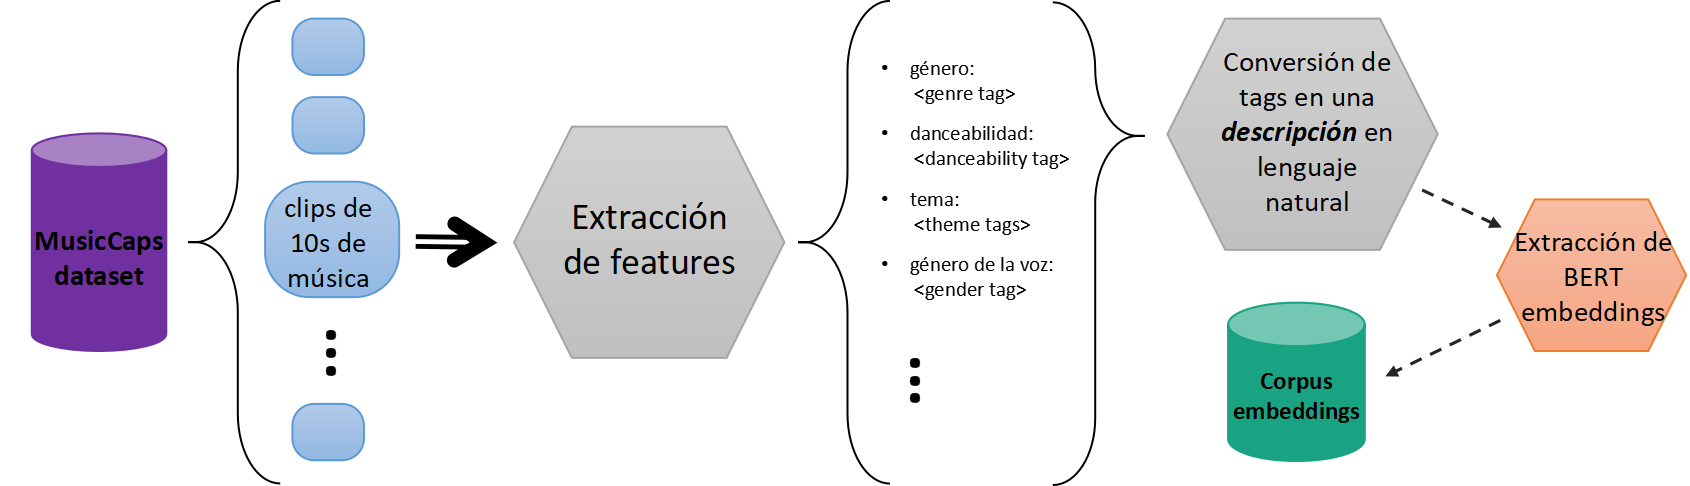
\includegraphics[width=\textwidth]{Graphics/corpus_embeddings.png}
	\caption{Diseño propuesto.} 
    \label{fig:corpus_embeddings}
\end{figure}
En el apartado de recuperación de información, el sistema consiste en recopilar la consulta del usuario, generar el vector de \textit{embedding} con SBERT y encontrar las canciones más similares comparando el vector con el corpus de \textit{embeddings}, utilizando similitud de coseno. En la imagen \ref{fig:sri_design} se observa el diseño del SRI. 
\begin{figure}[h]
	\centering
	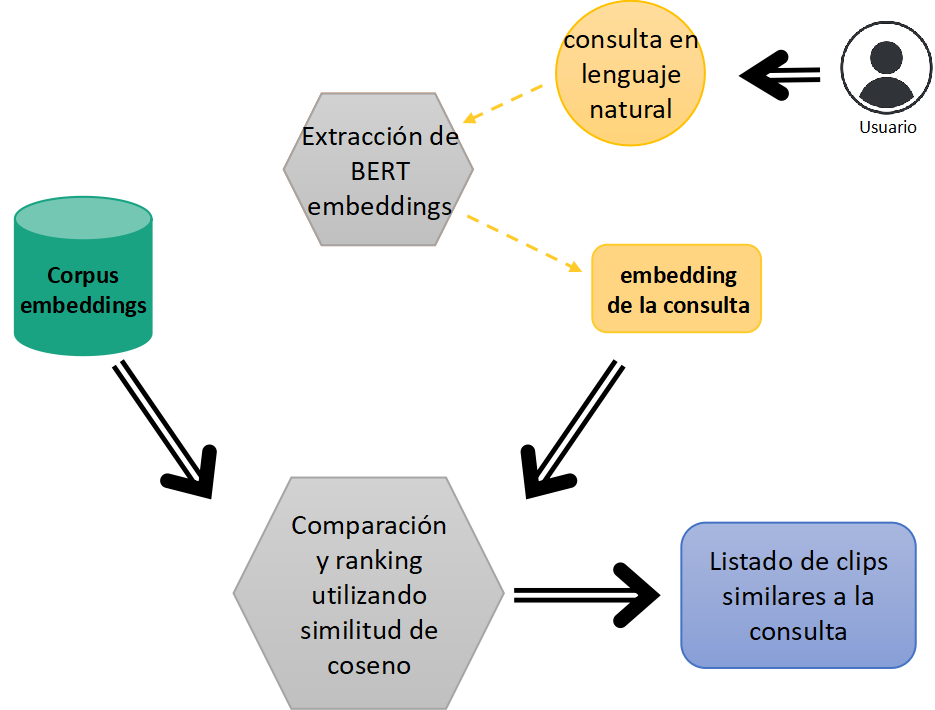
\includegraphics[width=0.6\textwidth]{Graphics/SRI.png}
	\caption{Sistema de recuperación utilizando \textit{Sentence BERT embeddings}.} 
    \label{fig:sri_design}
\end{figure}
\section{Detalles de implementación}
\label{sec:implementation}
\subsection{Extracción de \textit{features}}
\label{subsec:essentia}
La arquitectura del sistema de extracción de \textit{features} fue relativamente sencilla de implementar. Un sistema de clases que heredan de la clase abstracta \textit{FeaturesExtractor}. \\
Las propiedades incluyen: una lista de las etiquetas de clase posibles de cada modelo; \textit{feature\_description} que retorna una oración en lenguaje natural describiendo una etiqueta de clase; \textit{feature\_tags\_description} retorna un \textit{tag}/metadato describiendo una etiqueta de clase. Además de la función \textit{extract\_feature}, que recibe un clip de música y retorna el(los) \textit{feature(s)} extraídos con el modelo específico. \\
Los modelos utilizados, para probar y evaluar el diseño son parte de los que provee la biblioteca \textit{essentia} en conjunto con \textit{tensorflow} \cite{alonso2020tensorflow}. Se utilizaron 9 modelos : \href{https://essentia.upf.edu/models.html#genre-discogs400}{Genre Discogs400}, \href{https://essentia.upf.edu/models.html#mtg-jamendo-genre}{MTG-Jamendo genre},  \href{https://essentia.upf.edu/models.html#danceability}{Danceability}, \href{https://essentia.upf.edu/models.html#mood-happy}{Mood Happy}, \href{https://essentia.upf.edu/models.html#mood-relaxed}{Mood Relaxed}, \href{https://essentia.upf.edu/models.html#mood-sad}{Mood Sad}, \href{https://essentia.upf.edu/models.html#mtg-jamendo-mood-and-theme}{MTG-Jamendo mood and theme}, \href{https://essentia.upf.edu/models.html#mtg-jamendo-instrument}{MTG-Jamendo instrument} y \href{https://essentia.upf.edu/models.html#voice-gender}{Voice gender}.

Los modelos de clasificación de \textit{essentia} requiren que el audio sea convertido a \textit{embeddings} para recibirlos como entrada, y fue utilizado para ello el modelo \textit{Discogs-EffNet} \footnote{\href{https://essentia.upf.edu/models.html}{https://essentia.upf.edu/models.html}}.

En \textit{musiccaps-subset-feat.csv} \footnote{\href{https://github.com/NileyGF/Busqueda-semantica-en-audios.-Tesis/blob/main/src/data/musiccaps-subset-feat.csv}{https://github.com/NileyGF/Busqueda-semantica-en-audios.-Tesis/blob/main/src/data/musiccaps-subset-feat.csv}} (tabla \ref{tab:feat.csv}) se puede observar el subconjunto utilizado de MusicCaps con los \textit{features} extraídos, además de la información originaria del dataset sobre cada clip. Este proceso, en una computadora con 24 GB de RAM y procesador Intel Core i7-4710HQ, tomó alrededor de 18 horas para terminar con los alrededor de 3800 clips.
\begin{table}[h]
    \tiny
    \centering
    \begin{tabular} { | p{5em} | p{4em} | p{6em} | p{4em} | p{4.5em} | p{4.5em} | p{4em} | c | p{4.8em} | p{4em} |}
    \hline
     \multicolumn{3}{|c|}{ } & \multicolumn{7}{|c|}{Extracted features} \\
    \hline
        ytid    & aspect list & caption &Discogs 400 genre & MTG Jamendo genre &danceability & happy & ... &instruments & voice gender\\ 
    \hline
    -0Gj8-vB1q4 &['low quality', ... , 'ballad'] &"The low quality recording ... like something you would hear at Sunday services." & 
                                    Stage \& Screen---Soundtrack & classical &not danceable &non happy & ... & ['piano', 'violin', 'cello'] & female \\
    \hline
    -0SdAVK79lg &['guitar song', 'piano backing', ... , 'no voice'] &"This song features an electric guitar ... This song can be played in a coffee shop."  
                                &Blues---Delta Blues & pop &not danceable & non happy & ... & ['guitar', 'acousticguitar', 'bass'] & female \\
    \hline
    \multicolumn{10}{|c|}{ \textbf{.....} } \\ 
    \hline
    \end{tabular}
    \caption{Fragmento del archivo musiccaps-subset-feat.csv}
    \label{tab:feat.csv}
\end{table}

\subsection{Conversión de tags en una descripción en lenguaje natural}
\label{subsec:feat-to-text}

Como fue mencionado en la sección \ref{sec:design}, la idea era implementar tres alternativas para obtener descripciones a partir de los \textit{features} extraídos anteriormente. \\

\textbf{Utilizar GPT-2 con \textit{prompt engineering}}\\
Se intentó unas decenas de prompts utilizando el modelo de completamiento de texto de GPT-2 \cite{radford2019language, HggFaceGPT2}. Sin embargo, no se obtuvo resultados aceptables con ningún de ellos. Teniendo en cuenta dichos resultados se probó con GPT-3.5, desde la página de Open-AI; y esta vez si se observaron buenas descripciones, aunque no completamente fieles, como es de esperar de estos modelos. Sin embargo, no es factible realizar casi 4000 peticiones, ya que a diferencia de GPT-2, GPT-3.5 no es tan accesible. Por lo tanto esta alternativa tuvo que ser descartada.\\

\textbf{Crear una oración con fuerza bruta}\\
Utilizando la propiedad \textit{feature\_description}, se generó una oración por cada \textit{feature} extraído, por cada uno de los clips en el dataset. La concatenación de dichas oraciones en un texto constituyó el corpus de descripciones. \\
Ejemplos de la metodología para crear las oraciones:
\begin{itemize}
    \item MTG-Jamendo genre: " The music genre sounds like <\textit{genre classification}>. "
    \item Mood Relaxed: $"$ Its sound is >\textit{relaxing/not relaxing}>. "
    \item MTG-Jamendo instrument: " You can hear the sounds of <\textit{comma separated top instruments}>. "
    \item Voice gender: " There is a <\textit{female/male}> voice. "
\end{itemize}
Aprovechando la libertad al diseñar el sistema de recomendación, se propuso realizar un segundo corpus de descripciones conteniendo las oraciones separadas además del texto resultado de la concatenación. De forma que este corpus extendido tiene 10 descripciones (que posteriormente son transformadas en \textit{embeddings}) por cada clip (una oración por cada uno de los 9 \textit{features} y el texto completo). Esta idea surge para comparar que ofrece mejores resultados en la recuperación con \textit{embeddings}: una consulta en forma de texto largo u oraciones más cortas, pero repetitivas a través del conjunto de datos.\\

\textbf{Concatenar \textit{features} sin intentar que parezca una oración humana}\\
Utilizando la propiedad \textit{feature\_tags\_description}, se creó una `oración' por cada clip, donde el valor de cada \textit{feature} es separado del siguiente por un `; '. En algunos, la propiedad modifica ligeramente el valor resultante del modelo de clasificación. Por ejemplo, tiene más sentido semántico utilizar \textit{``\{female/male\} voice ''}, que simplemente \textit{``\{female/male\}''}.\\

En \textit{musiccaps-subset-descriptions.csv} \footnote{\href{https://github.com/NileyGF/Busqueda-semantica-en-audios.-Tesis/blob/main/src/data/musiccaps-subset-descriptions.csv} {https://github.com/NileyGF/Busqueda-semantica-en-audios.-Tesis/blob/main/src/data/musiccaps-subset-descriptions.csv } } (tabla \ref{tab:descriptions.csv})  se pueden observar las descripciones de cada clip, tanto en formato de oraciones procesadas, como de tags concatenados. 
\begin{table} [h]
    \tiny
    \centering
    \begin{tabular} { | p{5em} | p{4em} | p{6em} | p{4em} | p{4em} | c | p{4em} | p{6em} | p{6em} |}
    \hline
     \multicolumn{3}{|c|}{ } & \multicolumn{4}{|c|}{Extracted features} & \multicolumn{2}{|c|}{Descriptions} \\
    \hline
        ytid    & aspect list & caption &Discogs 400 genre & MTG Jamendo genre & ... & voice gender & description & tags description \\ 
    \hline
    -0Gj8-vB1q4 &['low quality', ... , 'ballad'] &"The low quality recording ... like something you would hear at Sunday services." & Stage \& Screen---Soundtrack & classical & ... & female &"The music genre is considered to be Stage \& Screen, Soundtrack ... There is a female voice. " &"Stage \& Screen, Soundtrack; classical; ... ; female voice."\\
    \hline
    -0SdAVK79lg &['guitar song', 'piano backing', ... , 'no voice'] &"This song features an electric guitar ... This song can be played in a coffee shop."  & Blues---Delta Blues & pop & ... & female &"The music genre is considered to be Blues, Delta Blues ... There is a female voice. " &"Blues, Delta Blues; pop; ... ; female voice."\\
    \hline
    \multicolumn{9}{|c|}{ \textbf{.....} } \\ 
    \hline
    \end{tabular}
    \caption{Fragmento del archivo musiccaps-subset-descriptions.csv}
    \label{tab:descriptions.csv}
\end{table}

\subsection{Extracción de \textit{embeddings} de BERT}
\label{subsec:bert-embedd-extr}

Cada uno de los 3 corpus de descripciones fueron posteriormente procesados para crear un vector de \textit{embeddings} por cada clip utilizando el modelo de la biblioteca \textit{transformers} de \textit{HuggingFace}: \textbf{bert-base-uncased}. El proceso consiste en tokenizar el texto con la función \textbf{BertTokenizer} de \textit{transformers}: \\
\begin{lstlisting}[language=Python]
preprocess_tokens = "[CLS]" + text + "[SEP]"
\end{lstlisting} 
Luego se transforma el texto tokenizado a \textit{embeddings}, utilizando la biblioteca \textit{torch} y el modelo de BERT. Al finalizar se guarda la lista de embeddings como un archivo binario, que no se encuentran en el repositorio debido a que ocupan relativamente bastante espacio.

El primer corpus de \textit{embeddings} tomó en computarse, en una computadora con 24 GB de RAM y procesador Intel Core i7-4710HQ, alrededor de 2 horas. El segundo, que consiste en una extensión del primero con 10 veces la cantidad de \textit{embeddings}, tomó entre 14 y 15 horas de procesamiento. El tercer corpus, constituido por la concatenación de tags tomó entre 1 y 2 horas en terminar.

Como último detalle, en esta parte de la implementación al finalizar de procesar cada corpus se creó un diccionario que establece por cada \textit{embedding} a que clip corresponde. Esto es particularmente importante en el caso del segundo, ya que existen 10 \textit{embeddings} por cada clip.

\subsection{Recuperación de Información. Comparación y ranking}
\label{subsec:IR-process-query}

El método de obtener la música más cercana consiste en obtener un vector de \textit{embeddings} a partir del texto de la consulta, utilizando el mismo proceso descrito anteriormente en  \ref{subsec:bert-embedd-extr}. Luego se compara dicho vector con cada uno de los \textit{embeddings} en el corpus (solo se emplea uno de los tres), utilizando la similitud del coseno entre el ángulo de los vectores. Finalmente se ordenan descendentemente, ya que el coseno es mayor entre vectores más cercanos. Se puede especificar cuantos resultados obtener: todos, o solo los $k$ más similares a la consulta. 

Después de ordenar los \textit{embeddings} se busca la correspondencia entre ellos y los clips, de forma que la relevancia de un clip es la relevancia del primer \textit{embedding} correspondiente a él (o sea, el de mayor valor de coseno). Esto es particularmente importante para el segundo corpus y cualquier otro que se pueda diseñar eventualmente donde a un clip le corresponda más de un vector de \textit{embeddings} (por ejemplo, si la descripción contiene más de 512 \textit{tokens} no puede ser procesada con BERT, y puede solucionarse dividiéndola en varias subdescripciones más cortas).


%===================================================================================
% Chapter: Experimentation
%===================================================================================
\chapter{Breve Experimentación}
\label{chap:experiment}
%===================================================================================

\section{Consideraciones generales}
\label{sec:consid}
Para evaluar un SRI, tradicionalmente, se parte de un conjunto de documentos y un conjunto de consultas con una relación de relevancia establecida entre ambos \cite{manning2008introductiontoIR}. Esta relación es fundamental para identificar los elementos relevantes para una consulta, e incluso puede determinar el grado de relevancia. Algunos ejemplos de datasets para evaluar SRIs son: \href{https://ir-datasets.com/antique.html}{\textit{antique}}, \href{https://ir-datasets.com/car.html}{\textit{car}}, \href{https://ir-datasets.com/cranfield.html}{\textit{cranfield}}, \href{https://ir-datasets.com/msmarco-passage.html}{\textit{msmarco-passage}}, \href{https://ir-datasets.com/nfcorpus.html}{\textit{nfcorpus}}, \href{https://ir-datasets.com/nyt.html}{\textit{nyt}}.

Las estrategias de evaluación centradas en el usuario buscan tener en cuenta diferentes factores en la percepción de las cualidades musicales, en particular de la similitud musical. Esto es especialmente importante ya que las nociones de similitud musical están probremente definidas. El acuerdo entre los humanos sobre el parecido entre dos piezas musicales está limitado a alrededor del 80\% según se afirma en la literatura \cite{Schedl2014MusicIR}.\\
En general los SRIs evalúan la semejanza utilizando la métrica de similitud de coseno \cite{Brundha2022VectorMB}. Esta técnica calcula la similitud entre dos elementos basándose en el ángulo entre sus representaciones vectoriales. Su popularidad se basa en que es invariante a la magnitud del vector, es eficiente de computar y que en epacios multi-dimensionales captura la orientación de los datos.

Un gran número de estudios de recuperación de información han demostrado que los usuarios de los sistemas de recuperación tienden a prestar atención, principalmente, a los primeros resultados \cite{Mitra2017NeuralMF}. Por lo tanto, las métricas de recuperación de información se centran en comparaciones basadas en los primeros resultados recuperados. Estas métricas generalmente se calculan en una posición, digamos $k$, y luego se promedian sobre todas las consultas.

El hecho de que no existen datasets de recuperación de información de música implica que en todos los experimentos en el tema se definen las consultas y la relevancia entre una consulta y la música de forma diversa.

Utilizando la información proveída por el dataset (sec. \ref{sec:datasets}) fueron concebidos dos conjuntos de consultas. El primero con las descripciones creadas por músicos y el segundo con la lista de aspectos (convertida en oraciones concatenando los \textit{tags}). Durante el preprocesamiento se extraen los \textit{embeddings} de ambos conjuntos (utilizando SBERT \cite{Reimers2019SentenceBERTSE}) y se guardan en archivos binarios. \\
Es necesario establecer una relación de relevancia entre consultas y clips. Para ello fue diseñado un algoritmo que itera por los \textit{embeddings} de cada conjunto de consultas. \\
El algoritmo crea una lista $R$, donde para la consulta i-ésima:
\begin{lstlisting}[language=Python]
R[i] = [(song_id_1, cosine_similarity_i1), ... ,(song-id_j, cosine_similarity_ij)]
\end{lstlisting}
R[i] contiene una tupla por cada consulta $j$ que cumpla: $$cosine\_similarity(i,j) \geq 0.95$$ ya que se considera que a descripciones similares corresponden clips similares. De esta forma siempre se obtiene el clip que describe la consulta $i$ pues $cosine\_similarity(i,i) = 1$.
 
En \textit{Toward Universal Text-To-Music Retrieval} \cite{Doh2022TowardUT} se realiza uno de los análisis más recientes y abarcadores sobre modelos de recuperación de música utilizando texto. Ellos utilizan un subconjunto fijo de 1000 consultas para evaluar varios modelos; por lo que este trabajo considera mantener ese número.

Para ello se extrae un subconjunto aleatorio de 1000 consultas antes de cada proceso de evaluación. Se utilizó un \textit{seed} para que al ejecutar el proceso de evaluación se obtengan resultados consistentes. 

Debido a que fueron propuestos 2 conjuntos de consultas y 3 de descripciones (sec. \ref{subsec:feat-to-text}), cada experimento debe ser repetido 6 veces. El nombre de cada combinación se define como: $consultas-descripciones$ . Más detalles en la figura  \ref{alg:query-corpus}.
\begin{figure}[h!] 
\begin{lstlisting}[language=Python]
descripciones = {corpus: "Descripciones creadas generando oraciones a partir de feature_description y uniendolas en un texto descriptivo.",
                ext_corpus: "Extension del primer corpus; conteniene los mismos textos y las oraciones que lo componen separadas.",
                tag_corpus: "Consiste basicamente en la concatenacion de todos los features que retornan los modelos de la seccion \ref{subsec:essentia} por cada clip."}
consultas = {capt: "Columna \'caption\' del dataset MusicCaps, son descripciones textuales escritas por musicos.",
             aspect: "Esta conformado por la concatenacion de las etiquetas de la columna \'aspect list\' del dataset MusicCaps."}
\end{lstlisting}
\caption{Definición de los conjuntos de descripciones y consultas.} \label{alg:query-corpus}
\end{figure}

\section{Recobrado y precisión}
\label{sec:experiment1}
El primer experimento evalúa el recobrado (\textit{recall}) y la precisión promedio (\textit{mean average precision} mAP). El recobrado representa la proporción entre las canciones recuperadas que son relevantes y el número total de canciones relevantes. En particular se calcula el $recall@k$ con $k=$1, 5, 10, 50; que solo considera los primeros $k$ elementos recuperados. El mAP promedia los resultados de precisión en cada rango donde se encuentra un clip relevante \cite{mAPAnalyticsYogi}. La precisión representa la fracción de elementos recuperados que son relevantes para la consulta del usuario. Esta métrica se ha utilizado durante mucho tiempo como el “estándar de oro” de facto para la evaluación de sistemas de recuperación \cite{Beitzel2009}. Se calcula el mAP general y mAP@10 (donde se consideran solo los top 10 clips recuperados). 

Todas las métricas se calculan para cada consulta y luego se promedian resultando en los valores que se muestran en la tabla \ref{tab:results}.

\begin{table}[h]
    \footnotesize
    \centering
    \begin{tabular} { | l | c | c | c | c | c | c | }
    \hline
                      &   R@1           &   R@5   &   R@10         &   R@50          & mAP@10        &   mAP   \\ 
    \hline
    capt-corpus       & 0.00082         & 0.00499 & 0.0096         & 0.03492         & 0.107         & 0.0352 \\
    capt-ext\_corpus   & 0.00076         & 0.0059  & 0.0095         & 0.03485        & 0.101         & 0.0357  \\ 
    capt-tag\_corpus   & 0.00025         & 0.00202 & 0.0057         & 0.0273         & 0.075         & 0.0374  \\ 
    aspect-corpus     & 0.00124         & 0.0047  & 0.0117         & 0.0424          &\textbf{0.124} & 0.0296 \\ 
    aspect-ext\_corpus &\textbf{0.00137} & 0.0053  & 0.0098         & 0.0344         & 0.078         & 0.028 \\ 
    aspect-tag\_corpus & 0.00056 &\textbf{0.00761} &\textbf{0.01254} &\textbf{0.0524} & 0.096 &\textbf{0.0381} \\ 
    \hline
    \end{tabular}
    \caption{Resultados de las 6 combinaciones consultas-corpus	respecto a recall y mean average precision.}
    \label{tab:results}
\end{table}

Se observa que, en general, utilizar el \textit{aspect list} como consultas provee mejores resultados, en particular cuando se utiliza como corpus los \textit{tags} concatenados. Además el mAP, que se supone que es muy representativo, tiene mejores valores que el recobrado. En cuanto a las consultas que consisten en las descripciones creadas por expertos, los mejores valores se obtienen con el corpus conformado por un texto descriptivo por cada clip. 

También se ilustra que tanto el par de consultas-de-texto-descriptivo, corpus-de-texto-descriptivo; como el par de consultas-de-tags-concatenados, corpus-de-tags-concatenados; resultaron en los mejores valores. Esto puede indicar que es mejor que el corpus a utilizar para describir la música tenga la forma que más prevalece en las consultas de los usuarios. 

\section{Índice de aciertos}
\label{sec:experiment2}

El segundo experimento evalúa una métrica no muy común, pero que refleja de forma simple un factor importante para los usuarios. Fue calculado el índice del modelo de mostrar elementos relevantes en los primeros $k$ clips recuperados (para $k$ que refleja cuantos resultados usualmente comprueban los usuarios (1, 5, 10) ). \\
Entonces el \textit{$hits\_rate@k$} para una consulta tiene como valor 1 si en los primeros $k$ resultados hay algún clip relevante y 0 si no. Finalmente se promedia, para un $k$ fijo, todos los \textit{$hits\_rate@k$}, obteniendo el índice de consultas donde en los top $k$ resultados se recuperan buenos clips.

\begin{table}[h]
    \footnotesize
    \centering
    \begin{tabular} { | l | c | c | c | c | }
    \hline
                       &   hits\_rate@1   &   hits\_rate@5   &  hits\_rate@10 \\ 
    \hline
    capt-corpus        & 0.052           &  0.193          &  \textbf{0.333}  \\
    capt-ext\_corpus   & 0.05            &  0.182          &  0.314          \\ 
    capt-tag\_corpus   & 0.027           &  0.142          &  0.248          \\ 
    aspect-corpus      & \textbf{0.087}  &  \textbf{0.215} &  0.301          \\ 
    aspect-ext\_corpus & 0.052           &  0.137          &  0.209          \\ 
    aspect-tag\_corpus & 0.037           &  0.18           &  0.303          \\ 
    \hline
    \end{tabular}
    \caption{Resultados de las 6 combinaciones consultas-corpus	respecto al índice de aciertos.}
    \label{tab:hitsresults}
\end{table}

En la tabla \ref{tab:hitsresults} se observa que los resultados para esta métrica son bastante uniformes y los mejores valores se obtienen con el corpus número 1. Con la lista de aspectos como consultas y el primer corpus se obtiene casi el doble de resultados relevantes en la primera posición que con el resto. \\
Además, atendiendo a la motivación de este experimento se obtuvo que aproximadamente un tercio de las consultas tienen un clip relevante entre los primeros 10 (de más de 3800 clips). 

\section{Discusión}
\label{sec:final-discution}
Se pudo observar que, en ambos experimentos, no se obtienen resultados muy distintos entre \textit{corpus} y \textit{ext\_corpus}. Lo que conlleva a concluir que del texto se infiere aproximadamente la misma información semántica que de las oraciones que lo componen. El hecho de procesar un corpus 9 veces más grande (en este caso porque solo se utilizaron 9 modelos) aumentó el tiempo de extracción de \textit{embeddings} y el de recuperación considerablemente. Por lo que se debe considerar que no es una buena estrategia aumentar el corpus como se propuso. 

% Al momento de comparar nuestros resultados con los de MuLan \cite{Huang2022MuLanAJ}, MusCALL \cite{Manco2022ContrastiveAL} y Contrastive, Triplet Sentence BERT \cite{Doh2022TowardUT} es muy importante tener en cuenta que la única similitud entre los trabajos es que la tarea es recuperación de música utilizando consultas en lenguaje natural. 
Antes de considerar comparar los resultados obtenidos con otras investigaciones hay que tener en cuenta que ninguna utliza el mismo conjunto de música ni de consultas. Tampoco se comparte la estrategia de recuperación ya que los modelos de MuLan \cite{Huang2022MuLanAJ}, MusCALL \cite{Manco2022ContrastiveAL} y Contrastive Sentence BERT \cite{Doh2022TowardUT} utilizan modelos de aprendizaje contrastivo. Debido a lo novedoso de la estrategia propuesta en este trabajo y al problema que existe en el campo de recuperación de música a partir de texto respecto a la falta de datasets y la ausencia de un protocolo uniforme para la evaluación multimodal, no es factible hacer una comparación que lance alguna conclusión significativa ya que no hay puntos comunes. Sin embargo se espera que, con la publicación de MusicCaps \cite{Agostinelli2023MusicLMGM} y otros datasets en el futuro, surjan nuevas investigaciones o se reevaluen modelos existentes con métricas y datos comunes. 

%===================================================================================
% Chapter: Conclusions
%===================================================================================
\chapter*{Conclusiones}
\label{chap:conclusions}
\addcontentsline{toc}{chapter}{Conclusiones}
%===================================================================================
Esta tesis presentó un enfoque para la recuperación de música con consultas en lenguaje natural, que aprovecha el poder de los clasificadores de MIR y los \textit{embeddings} de oraciones.

A través de la exploración, se ha mostrado el potencial de utilizar clasificadores de aprendizaje automático (\textit{machine learning}) para extraer características matizadas de la música, en un intento de traducir sus cualidades auditivas en una descripción en lenguaje natural. Este paso representa un puente crítico entre la naturaleza abstracta de la música y el ámbito lingüístico de la comunicación humana, reduciendo la brecha semántica y allanando el camino para mejores sistemas de recuperación de música. Ahí radica la importancia de continuar por esta vertiente de investigación y encontrar otras formas de realizar la transformación de las características musicales a textos de que representen la percepción humana. Es probable que una forma de mejorar en este esfuerzo sea siguiendo los grandes avances en modelos de lenguaje de los últimos años (ya sea TableGPT u otro enfoque).

%Nuestra investigación resalta el potencial de aplicaciones prácticas dentro de la industria musical, sugiriendo un enfoque que podría revolucionar la forma en que los usuarios interactúan y descubren la música. Desde recomendaciones personalizadas hasta interfaces de búsqueda más intuitivas, el impacto de esta investigación se extiende más allá del ámbito académico, resonando profundamente dentro del campo de la tecnología musical.

Es importante reconocer las limitaciones del trabajo. Aunque el prototipo es prometedor, todavía existen desafíos por abordar, como la interpretabilidad de las descripciones en lenguaje natural y la escalabilidad del proceso de recuperación. También es importante señalar que aún no existen datasets para la tarea de recuperación de texto a música, y los datasets adaptables para la tarea no son de un tamaño adecuado. 
Se reconoce que las causas de la indisponibilidad de datasets también deben abordarse. Entre ellas se encuentran: el problema mencionado de los derechos de autor (\textit{copyright}), el hecho de que la alineación de texto y audio es una tarea computacional difícil que debe ser supervisada por humanos, y la ausencia de un estándar ampliamente adoptado para la representación multimodal de la música. Enfoques recientes de aprendizaje de representaciones multimodales han mostrado avances en muchos dominios al aprovechar enormes datos de la web, pero no en dominios musicales (al menos no en investigaciones públicas).

El potencial para futuros avances en la recuperación de música y sistemas de recomendación es vasto. Se espera que esta investigación siente las bases para estos esfuerzos futuros. Este es un primer intento de construir una interfaz de lenguaje natural de forma libre para música, y hay mucho espacio para mejorar.

%===================================================================================
% Chapter: Recommendations
%===================================================================================
\chapter*{Recomendaciones}
\label{chap:recommendations}
\addcontentsline{toc}{chapter}{Recomendaciones}
%===================================================================================

En vista a futuras investigaciones se recomienda utilizar TableGPT \cite{Gong2020TableGPTFT} u otro modelo de \textit{table-to-text generation} para la tarea de obtener una descripción de la música a partir de una lista de \textit{features}. Para comparar el resultado con los presentados en este trabajo, que utilizan un acercamiento de fuerza bruta. \\
Otra idea a incorporar es aumentar la cantidad y diversidad de modelos de clasificación en el sistema de extracción de \textit{features} (sec. \ref{subsec:essentia}). Debería resultar en un prototipo más eficiente.

En la sección de discusión de los resultados de la experimentación (sec. \ref{sec:final-discution}) se plantea que \textit{ext\_corpus} no es una alternativa factible para mejorar las descripcioes. Sin embargo, se podría evaluar un corpus conformado por un par de vectores de \textit{embeddings} por cada canción: uno de descripciones en forma de texto y otro formado por tags (o sea, una combinación de las ideas del primer y el tercer corpus propuesto). Además, en el experimento 1 (sec. \ref{sec:experiment1}) se analiza que los resultados mejoran cuando las consultas tienen la misma forma que las descripciones. Un corpus mixto puede ser una solución robusta al hecho de que no se puede preveer que tipo de consulta utilizarán los usuarios en la búsqueda.

Para finalizar se recomienda evaluar el prototipo realizando estudios de ablación para comprobar el impacto de cada parte del sistema. Por ejemplo, cuánto mejoran los resultados al incluir la búsqueda utilizando \textit{embeddings} de BERT en comparación con el modelo vectorial (de bolsa de palabras) tradicional.


\backmatter

\bibliographystyle{unsrt}
\bibliography{Bibliography}

\end{document}